% Chapter 1

\chapter{Project 1: Binary Search} % Main chapter title

\label{Chapter1} % For referencing the chapter elsewhere, use \ref{Chapter1} 

\lhead{Chapter 1. \emph{Binary Search}} % This is for the header on each page - perhaps a shortened title

%----------------------------------------------------------------------------------------

\section{Implementations}
This project experiments with different binary search algorithms. All our implementations takes a sorted static array of integers as input, search
this using a varying query value and returns the value if found or the next highest value in the array if not found.
The different implementations all have a setup method called \verb!createDataStructure! and a search method called \verb!binSearch!.
We only measure the execution of the \verb!binSearch! methods as our implementations assume a static input array.
\begin{lstlisting}
  void createDataStructure(int* arr, int arrSize);
  int binSearch(int elem);
\end{lstlisting}

A binary search algorithm runs in $O(\log(n))$, where $n$ is the array size.
The following four implementations of the binary search algorithm used four different memory layouts. The tree structures are shown in figure \ref{fig:memory_layouts}.

\begin{figure}[htbp]
	\centering
		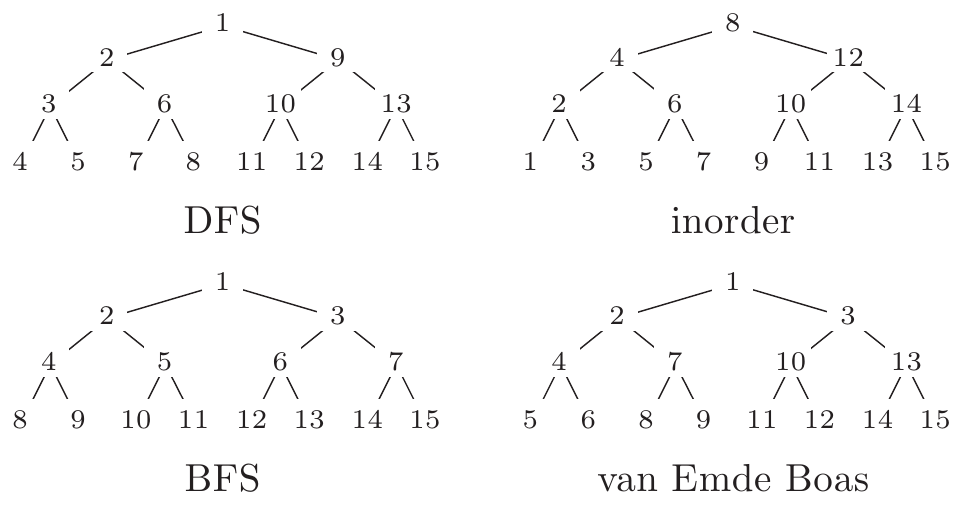
\includegraphics[width=\textwidth]{./Figures/Project1/MemoryLayouts.png}
		\rule{35em}{0.5pt}
	\caption[Memory layouts]{
	The four different tree structures shows the memory layout used in the implementations. The figure is taken from \citep{binAlg}.
	}
	\label{fig:memory_layouts}
\end{figure}


\subsection{Linear search}
To compare the running times for the algorithms, we have implemented a linear search function.
\begin{verbatim}
For each item in the list:
     if that item has the desired value,
         stop the search and return the item's location.
\end{verbatim}
 Return -1\footnote{We return -1 if the element dosn't exist in the list}.

\subsection{Inorder}

We have made a inorder binary search to compare with BFS, DFS and vEB.
Inorder is made iterative.
\lstinputlisting[language=C++, firstline=32, lastline=51, numbers=left]{./Figures/Project1/BinarySearch.cpp}
We begin by defining low, high and smallestSoFar.

In line 8 we make a while-loop, we run while high is greater than low.

We start by looking at the element whom is in the middle of the array.
If that element is smaller than the one we are looking for we set low to point at the middle +1.
If we are in the opposite case we set high to point at the middle -1.

The idea is that the array all the time is divided into one half the size where low will point at the first element in the new array and high will point at the last.

We continue until we find the element we are looking for or we return -1 if our list dosn't contain it.


\subsection{Breadth-first search (BFS)}
The following is a recursive method for filling out the bfs tree. The method is called by ``insert(0)''.
\begin{lstlisting}[numbers=left]
void insert(int bfsIndex){
  if (bfsIndex >= SIZE) return;
  insert(2*bfsIndex+1); // Left child
  bfsArray[bfsIndex] = *(linArray+linIndex);
  linIndex++;
  insert(2*bfsIndex+2); // Right child
}
\end{lstlisting}


The binary search is then implemented as follows:
\begin{lstlisting}[numbers=left]
  int i = 0;
  int curr = bfsArray[i];  // The current node visited
  int res = -1;  // The latest element smaller than 'elem'.
  while (curr != elem){
    i = 2*i+1;  // Left child
    if (curr < elem){
      i++;  // Right child (=left+1)
      res = curr;  // This is now the latest known element smaller than 'elem'.
    }
    // If we have reached a bottom node, return the last element lower than 'elem'.
    if (i >= SIZE){
      return res;
    }
    curr = bfsArray[i];
  }
  // At this point, the while loop did not continue because curr==elem
  return curr;
\end{lstlisting}



\subsection{Depth-first search (DFS)}
The implementation of depth first binary search (DFS) is based on \citep{binAlg}. 
The basic idea is to make a depth first traversal of the binary tree to create a different memory layout. 

The DFS implementation is build op like the other binary search implementations with a \verb!createDataStructure! and a \verb!binSearch! method. 
The \verb!createDataStructure! sets op the given sorted array in a DFS fashion and saves it in a new array, \verb!dfsArr!. 
The \verb!dfsArr! is created through a recursive method called \verb!dfsInsert!, that traverses the input array from left to right at insert in the \verb!dfsArr! in a recursive manner. 
The \verb!dfsInsert! method simulate traversal of the DFS tree and at each iteration of the tree-depth the method inserts the current element from the input array and then calls \verb!dfsInsert! on it's left and right children. 
\begin{lstlisting}[numbers=left]
void dfsInsert(int dfsIdx, int atDepth, int * inputArr) {
	if (dfsIdx < dfsArrSize && atDepth <= treeHeight) {
		int offset = floor(pow(2, (treeHeight - atDepth)));
		atDepth++;
		
		// Go left;
		dfsInsert(dfsIdx + 1, atDepth, inputArr);
		
		// Insert self	
		dfsArr[dfsIdx] = inputArr[insertFrom];
		insertFrom++;
		
		// Go right
		dfsInsert(dfsIdx + offset, atDepth, inputArr);
	}
} 
\end{lstlisting}
The left child is found by simply iterating one and the calculated \verb!offset! is used to find the left child. 
We observed that there is a relationship between two to the power of height of the tree and the current tree depth and index of the right child, 
and use this in the calculation of the offset.   

Making the actual binary search in the created DFS tree is done the same way as in the other algorithms, but also keeping track of the our current depth.
The highest value seen so far (lower than what we are looking for) is maintained and then the array is traversed like a binary tree. 
The main difference in DFS is what each time we need to visit the right child we calculate the \verb!offset! in same way as in \verb!createDataStructure!.  
But here shifting bits instead of using pow to save computation time (It could also been done this way in \verb!createDataStructure!, but we use \verb!pow! to ease the understanding). 
\begin{lstlisting}
 ...
// Go right
node = node + (1<<(treeHeight-atDepth));
...
\end{lstlisting}



\subsection{Van Emde Boas (vEB)}

The vEB array is constructed using the following recursive method. It is called using ``insert(0,0,0,roots)'' where roots is an array of the same size as the depth of the tree.

\begin{lstlisting}[numbers=left,escapeinside={@}{@}]
void insert(int vebIndex, int atDepth, int depthIndex, int roots[]){
  if (vebIndex >= size || vebIndex < 0) {
    return;
  }
  int rootIndex = findPosition((~atDepth+1) & atDepth); // returns the position of the rightmost 1-bit in "atDepth".
  int depthType = findPosition(~atDepth & (atDepth+1)); // returns the position of the rightmost 0-bit in "atDepth".
  int rootsNew[depth];
  for (int i=0; i<depth; i++){
      if (i <= rootIndex) rootsNew[i] = vebIndex;
      else rootsNew[i] = roots[i];
  }
  int amount = 1<<((1<<depthType)-1);  // 2^(2^depthType - 1)
  @\label{lst:vebLeft}@int vebLeft = (2*(depthIndex & (amount-1)) +1) * (2*amount -1) + rootsNew[depthType];  // (2*(depthIndex % amount)+1) * 2^(2^depthType) + "The root of the smallest local subtree"  insert(vebLeft, atDepth+1, 2*depthIndex, rootsNew); // Left child
  vebArray[vebIndex] = *(linArray+linIndex);
  linIndex++;
  int vebRight = vebLeft + 2*amount -1;
  insert(vebRight, atDepth+1, 2*depthIndex+1, rootsNew); // Right child
}
\end{lstlisting}

This vEB structure does not depend on the size of the input array. As a consequence, only inputs of size $2^{2^n}-1$ where $n$ is an integer generates fully balanced trees.
Otherwise it will always be more or less unbalanced, where the most of weight is located to the left. If for example the size is 9 then the left side will contain 7 elements compared to only 1 on the right side.
If we go one ``tree order'' further, if the size is 135, then there will be eight subtrees of size 15 each located to the of the root. That is, there will be 142 elements to the left of the root versus only 7 to the right.
In these two examples, almost half of the tree structure would not be utilized. Consequently, searching will on average require more iterations than balanced tree, since the tree is higher.
The worst case for this type of layout happens when the input size is $k 2^{2^n}$ where $2 < k \ll 2^{2^n}$. Then, more than half of the elements are located in the lower half of the tree, while at the same time, the tree is much higher than in a balanced tree.

The index calculation in line \ref{lst:vebLeft} is quite complex.
Some of the variables leading up to this calculation are illustrated in figure \ref{fig:vEB}.
\begin{figure}[htbp]
	\centering
		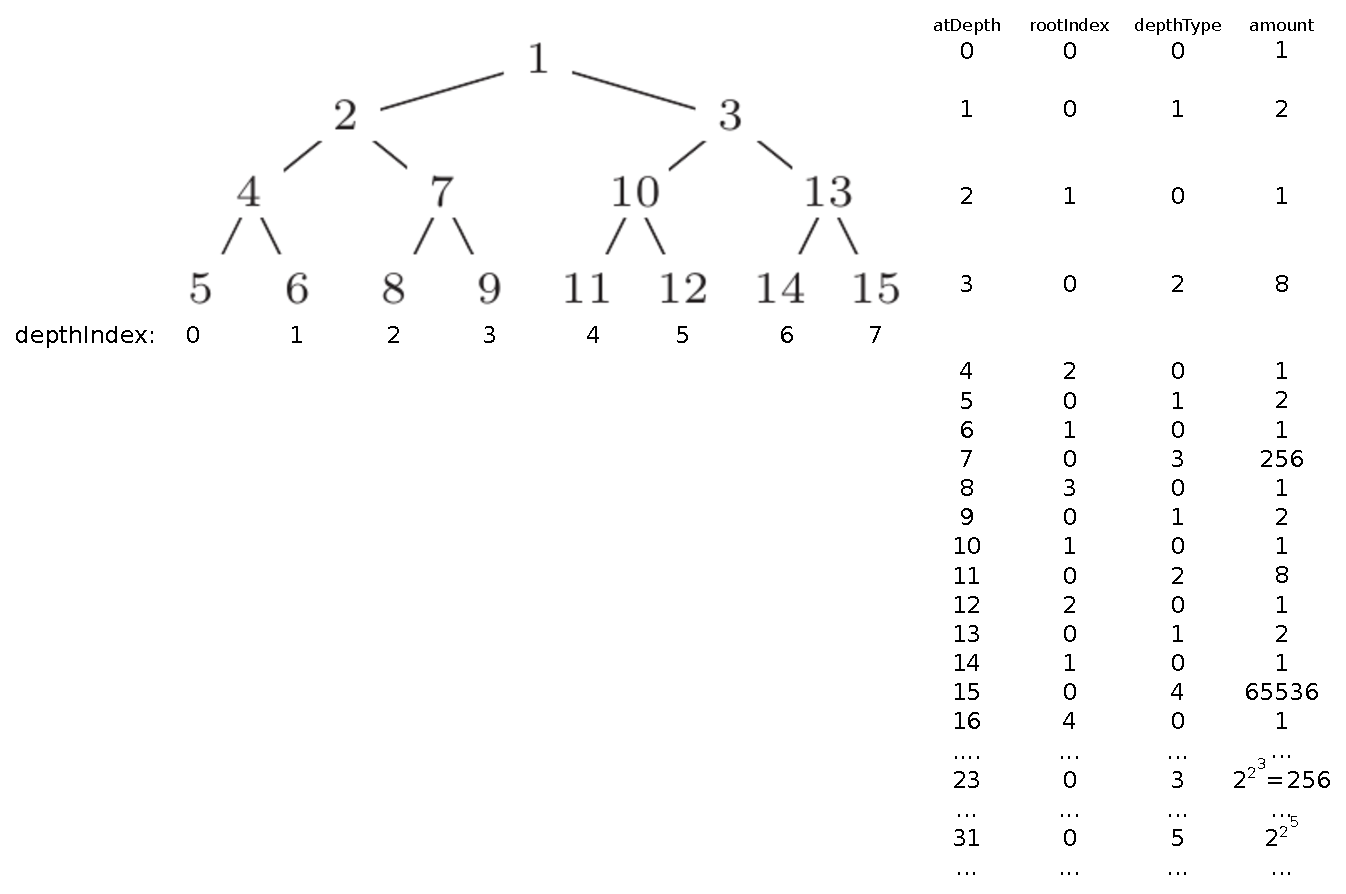
\includegraphics[width=\textwidth]{./Figures/Project1/vEB.eps}
		\rule{35em}{0.5pt}
	\caption[Van Emde Boas construction]{
	Bla bla bla.
	}
	\label{fig:vEB}
\end{figure}

First we do \verb!depthIndex&(amount-1)! which calculates how far to the right we are in the relevant subtree.
Then we double this value to find the number of new subtrees already placed by the neighbouring nodes to the left. One is added to take the current subtree into acount.
That value is now multiplied by the size of the current subtrees which is \verb!2*amount-1! to get the index of the left child in the parenting subtree.
Finally we add the index of root of the parenting subtree.


The binary search is implemented as follows:
\begin{lstlisting}[numbers=left,escapeinside={@}{@}]
  int vebIndex = 0;
  int curr = vebArray[vebIndex]; // The current node visited
  int res = -1; // The latest element smaller than 'elem'.
  int atDepth = 0;
  int depthIndex = 0;
  int roots[depth];
  for (int i=0; i<depth; i++){
      roots[i] = 0;
  }
  while (curr != elem){
    int rootIndex = ... // same as above
    int depthType = ...
    int amount = ...
    
    for (int i=0; i<=rootIndex; i++){
	roots[i] = vebIndex;
    }
    @\label{lst:veb_goRight}@int goRight = curr < elem;
    vebIndex = (2*(depthIndex & (amount-1)) +1 + goRight) * (2*amount -1) + roots[depthType];

    if (goRight){
      res = curr;  // This is now the latest known element smaller than 'elem'.
    }
    if (vebIndex >= size || vebIndex < 0){
      return res;  // we have reached the bottom of the tree.
    }
    atDepth++;
    depthIndex = 2*depthIndex + goRight;
    curr = vebArray[vebIndex];
  }
  // At this point, the while loop did not continue because curr==elem
  return curr;
\end{lstlisting}








\section{Results and discussion}

Looking at the branch misses in figure \ref{fig:Branch_misses_p1}, we see that three of the implementations have almost the same number of branch misses as a function of array size.
This follows intuitively from the fact that the trees are balanced and thus have the same height, and the number of branches are proportional to the height.
The vEB implementation, however, has a constant number of branch misses, no matter the size of the array. This is not caused by the unbalanced tree structure, since an even higher tree should produce at least as many branch misses.
Instead, it is caused by the specific way that the child index is calculated. Refering back to vEB binary search, when the comparison in line \ref{lst:veb_goRight} is used directly in the index calculation, the compiler uses a conditional move operation, thus eliminating the actual branch.

\begin{figure}[htbp]
	\centering
		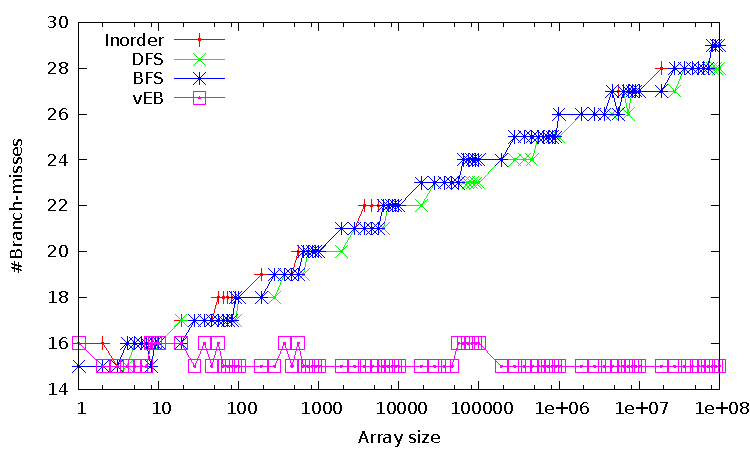
\includegraphics[width=\textwidth]{./Figures/Project1/Branch_misses.pdf}
		\rule{35em}{0.5pt}
	\caption[Branch misses]{
	The number of branch misses are plotted against the array size.
	}
	\label{fig:Branch_misses_p1}
\end{figure}


In figure \ref{fig:Cache_misses_p1}, the number of cache misses are shown. Inorder has the most cache refs and misses. This can be explained from the fact that searching the inorder array, jumps both forward and backwards.
In the other three layout, jumps only happen in the forward direction. 
Below an array size of about 64000 there are no cache refs or misses. The cache statistics indicates the use of the last level cache (L3).
The L3 cache is only used when the L2 cache is full. The test system has an L2 cache size of 256 kB, which corresponds to 64000 integers.
BFS has less cache refs and misses than DFS because finding the right child in DFS requires a significant jump forward.
vEB is designed to utilize the cache in the best possible way. When loading the value of a child chances are that the cached data contains some of the grandchildren.
So it is no surprise that it has the lowest cache misses and refs.

\begin{figure}[htbp]
	\centering
		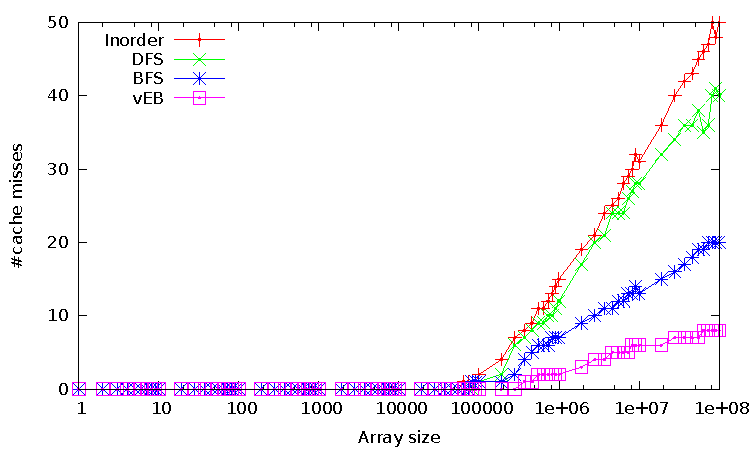
\includegraphics[width=\textwidth]{./Figures/Project1/Cache_misses.pdf}
		\rule{35em}{0.5pt}
	\caption[Cache misses]{
	The number of cache misses against array size.
	}
	\label{fig:Cache_misses_p1}
\end{figure}

\begin{figure}[htbp]
	\centering
		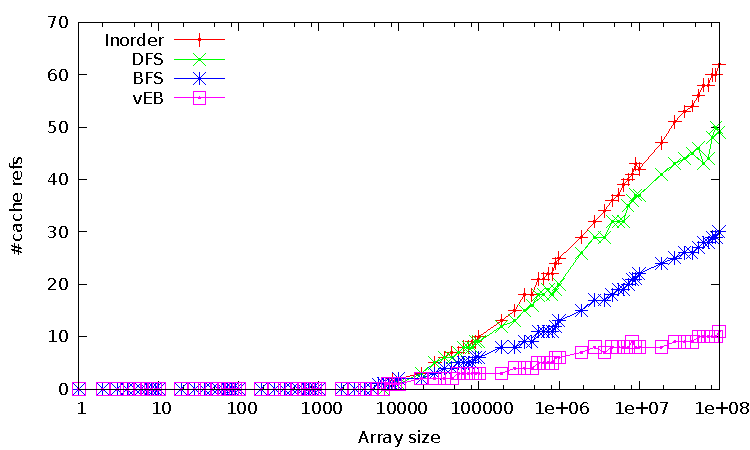
\includegraphics[width=\textwidth]{./Figures/Project1/Cache_refs.pdf}
		\rule{35em}{0.5pt}
	\caption[Cache refs]{
	The number of cache references against array size.
	}
	\label{fig:Cache_refs_p1}
\end{figure}

In figure \ref{fig:Instructions_p1} we see a peculiar behavior of the vEB. The overall course of the graph can be explained from the complex structure of the vEB which often generates very unbalanced trees.

\begin{figure}[htbp]
	\centering
		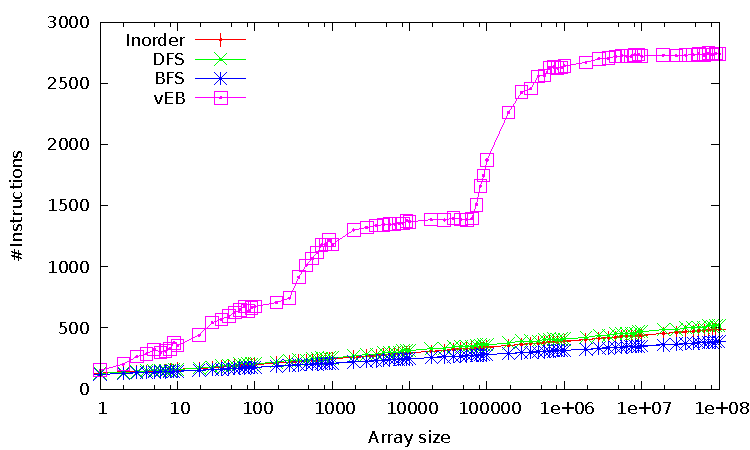
\includegraphics[width=\textwidth]{./Figures/Project1/Instructions.pdf}
		\rule{35em}{0.5pt}
	\caption[Instructions]{
	The number of hardware instructions plotted against array size.
	}
	\label{fig:Instructions_p1}
\end{figure}


The relationship between Inorder, BFS, and DFS corresponds nicely to the cache graphs. vEB, however, starts out being slower but catches up later on, for very large array sizes.
Looking at the cache graphs, we expected that the vEB was faster. The large amount of instructions could explain why it is slower than the others.
The spike at around 100000 can probably be attributed to some other processes taking up CPU time. This spike was not present in other runs.

\begin{figure}[htbp]
	\centering
		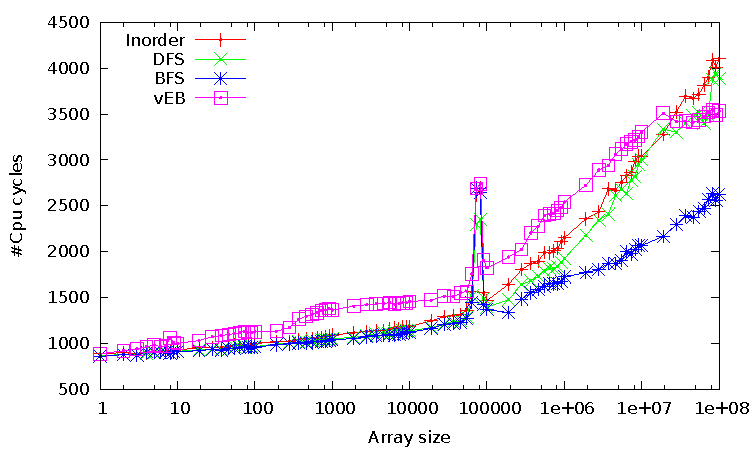
\includegraphics[width=\textwidth]{./Figures/Project1/Cpu_cycles.pdf}
		\rule{35em}{0.5pt}
	\caption[CPU cycles]{
	The number of CPU cycles plotted against array size.
	}
	\label{fig:Cpu_cycles_p1}
\end{figure}

